\begin{minipage}[t]{0.495\textwidth}
\centering
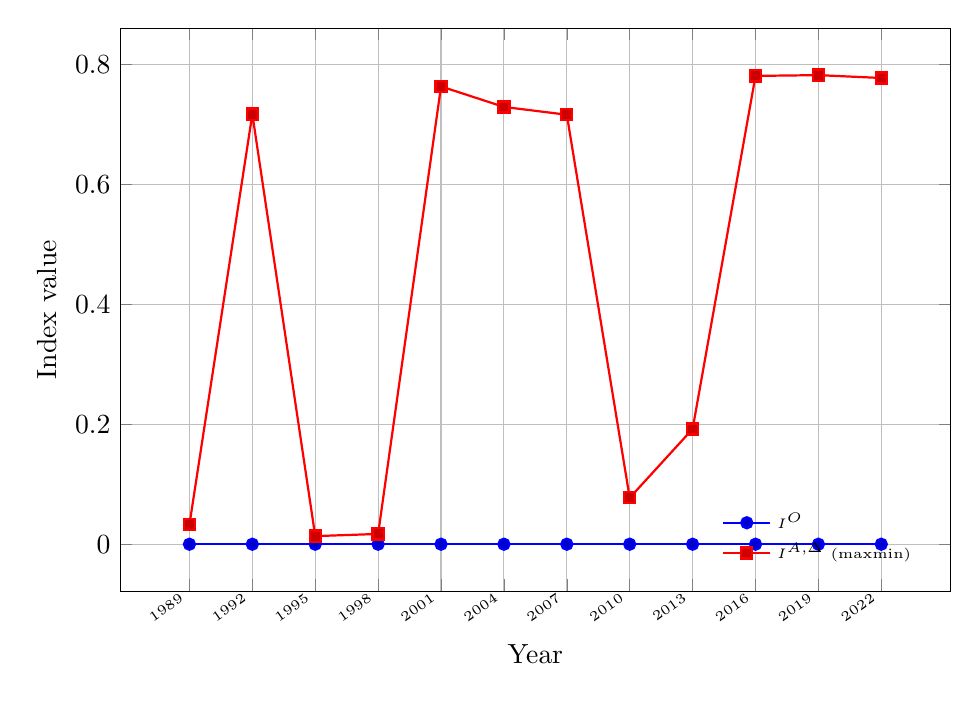
\begin{tikzpicture}
\begin{axis}[
width=\textwidth,
height=0.72\textwidth,
xlabel={Year},
ylabel={Index value},
legend pos=south east,
legend style={font=\tiny,draw=none,fill=none,cells={anchor=west}},
grid=major,
scaled x ticks=false,
xtick={1989,1992,1995,1998,2001,2004,2007,2010,2013,2016,2019,2022},
xticklabel style={/pgf/number format/fixed,/pgf/number format/precision=0,/pgf/number format/1000 sep={},rotate=35,anchor=east,font=\tiny},
]
\addplot+[thick, blue] coordinates {(1989, -0.00000000) (1992, -0.00000000) (1995, 0.00000000) (1998, 0.00000000) (2001, -0.00000000) (2004, -0.00000000) (2007, 0.00000000) (2010, 0.00000000) (2013, 0.00000000) (2016, 0.00000000) (2019, -0.00000000) (2022, 0.00000000)};
\addlegendentry{$I^{O}$}
\addplot+[thick, red] coordinates {(1989, 0.03276665) (1992, 0.71683594) (1995, 0.01349038) (1998, 0.01716064) (2001, 0.76295529) (2004, 0.72880220) (2007, 0.71580711) (2010, 0.07732820) (2013, 0.19206271) (2016, 0.78053021) (2019, 0.78179669) (2022, 0.77704166)};
\addlegendentry{$I^{A,\Delta}$ (maxmin)}
\end{axis}
\end{tikzpicture}
\end{minipage}
\hfill
\begin{minipage}[t]{0.495\textwidth}
\centering
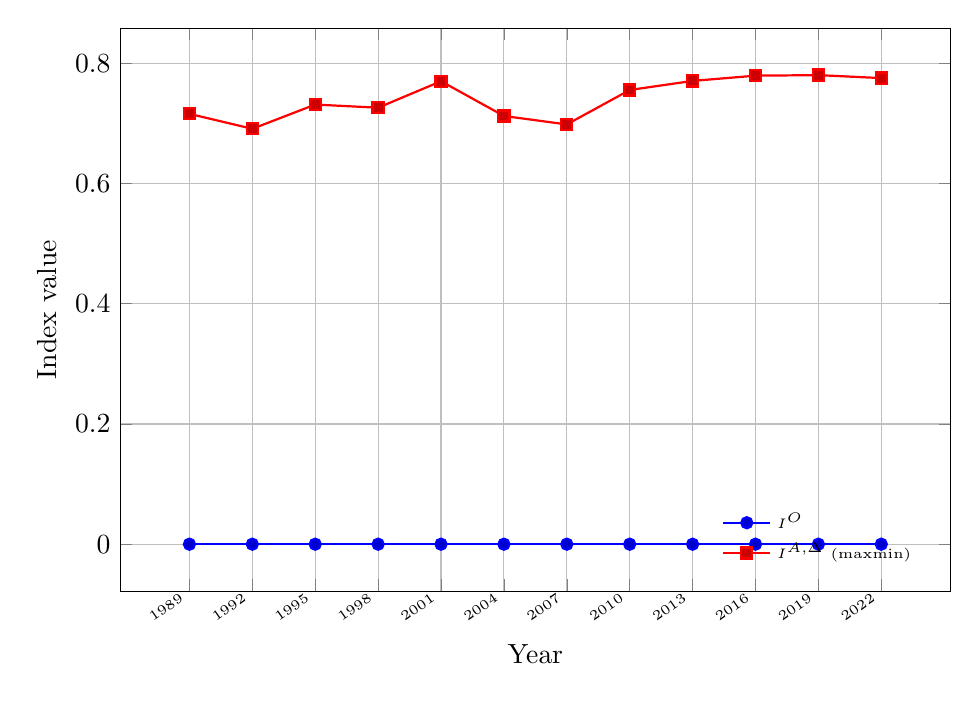
\begin{tikzpicture}
\begin{axis}[
width=\textwidth,
height=0.72\textwidth,
xlabel={Year},
ylabel={Index value},
legend pos=south east,
legend style={font=\tiny,draw=none,fill=none,cells={anchor=west}},
grid=major,
scaled x ticks=false,
xtick={1989,1992,1995,1998,2001,2004,2007,2010,2013,2016,2019,2022},
xticklabel style={/pgf/number format/fixed,/pgf/number format/precision=0,/pgf/number format/1000 sep={},rotate=35,anchor=east,font=\tiny},
]
\addplot+[thick, blue] coordinates {(1989, 0.00000000) (1992, 0.00000000) (1995, 0.00000000) (1998, -0.00000000) (2001, -0.00000000) (2004, -0.00000000) (2007, -0.00000000) (2010, 0.00000000) (2013, 0.00000000) (2016, -0.00000000) (2019, -0.00000000) (2022, 0.00000000)};
\addlegendentry{$I^{O}$}
\addplot+[thick, red] coordinates {(1989, 0.71589678) (1992, 0.69097789) (1995, 0.73134622) (1998, 0.72610830) (2001, 0.77016176) (2004, 0.71232894) (2007, 0.69829973) (2010, 0.75558326) (2013, 0.77068619) (2016, 0.77941483) (2019, 0.78029457) (2022, 0.77535078)};
\addlegendentry{$I^{A,\Delta}$ (maxmin)}
\end{axis}
\end{tikzpicture}
\end{minipage}

{\footnotesize $I^{A,\pi}$ with singleton $C=\{\pi_t\}$ equals $I^{O}$ (audit CSV: columns I\_O and I\_A\_singleton).}

% Gross Assets inequality measures
